%%%%%%%%%%%%%%%%%%%%%%%%%%%%%%%%%%%%%%%%%%%%%%%%%%%%%%%%%%%%%%%%%%%%%%%%
%                                                                      %
%     File: Thesis_Background.tex                                      %
%     Tex Master: Thesis.tex                                           %
%                                                                      %
%     Author: Andre C. Marta                                           %
%     Last modified :  2 Jul 2015                                      %
%                                                                      %
%%%%%%%%%%%%%%%%%%%%%%%%%%%%%%%%%%%%%%%%%%%%%%%%%%%%%%%%%%%%%%%%%%%%%%%%

%%%%%%%%%%%%%%%%%%%%%%%%%%%%%%%%%%%%%%%%%%%%%%%%%%%%%%%%%%%%%%%%%%%%%%
\chapter{State of the art}
\label{chapter:state}

In this chapter we present the state of the art of searches for Higgs pairs production at the LHC and  feasibility studies targeting searches for this process at future colliders. In addition, previous studies focusing on the granularity of the hadronic calorimeter as a key detector parameter are also reviewed.

In section \ref{section:previous_searches}, we review the searches that have been conducted at the LHC by the ATLAS and CMS experiments. We include discussions on the different final states that were targeted and report on the constraints that were derived for the di-Higgs cross section and trilinear coupling. A brief overview of the current constraints on some BSM models is also presented. In section \ref{section:feasibility}, we present the results obtained from feasibility studies that access the discovery potential for this process at the HL-LHC and at the FCC-hh. In section \ref{sec:gran}, we present previous studies on the impact of the granularity of the hadronic calorimeter on the spatial resolution of hadrons and on the resolution of the jet mass and of jet substructure observables.

\section{Searches for Higgs pair production at the LHC}
\label{section:previous_searches}
%
%IDEAS FOR SECTION
%
%- Previous searches by ATLAS and CMS at the LHC \checkmark\\
%- Different decay channels used: pros and cons + compare achieved sensitivities \checkmark \\
%Channels: bbbb, bb tau tau, bb gamma gamma, gamma gamma WW, bb ZZ \checkmark \\
%- Models investigated and motivation \\
%- Exclusion limits

%The discovery of the Higgs boson is a strong evidence that the Higgs mechanism operates in Nature. However, by itself, it does not guarantee that the shape of the Higgs potential is the one depicted in figure \ref{fig:higgsV}, on the right. In order to reconstruct the Higgs potential and gain a deeper understanding of the mechanism that leads to the breaking of the electroweak symmetry one must measure the Higgs boson self-couplings, namely its three and four point interactions, whose strengths depend on the values of the parameters of the Higgs potential, as shown in section \ref{eq:higgs_couplings}.  
%
%However, in the SM, the cross section for the production of Higgs pairs through ggF is extremely small: $\sim30~$fb at the current CM energy achieved at the LHC (value computed at Next to Leading Order (NLO) accuracy) \cite{higgsCrossSection}. This value is approximately three orders of magnitude smaller than the production cross section of a single Higgs boson. In addition, this value has to be multiplied by the branching fraction of the chosen decay channel which further reduces the effective cross section of the full process. Nonetheless, ATLAS and CMS have conducted searches for this process whose results are summarized in this section.

The searches performed so far at the LHC by ATLAS and CMS covered different decay channels and targeted not only the SM process but also some BSM scenarios where di-Higgs production is enhanced. Neither could achieve enough statistical significance to declare the measurement of this process in the SM nor have found any significant deviation from the expected values. These searches resulted in upper limits for the cross section of di-higgs production in the SM and for the values of the parameters of BSM benchmark theories. From the limits on the cross section it is also possible to constraint the values of the Higgs self coupling, $k_{\lambda}=\lambda_{hhh}/\lambda_{hhh}^{SM}$.

The $hh\rightarrow b\overline{b}b\overline{b}$ channel \cite{hh2bbbbATLAS,hh2bbbbCMS} benefits from the large branching fraction of $h\rightarrow b\overline{b}$ ($\sim 58 \%$). In addition, ATLAS showed that this is the most sensitive channel to resonance masses over $500$ GeV \cite{hhATLAS}. However, this channel suffers with an overwhelming multijet background which drives the need for very tight trigger level cuts in order to bring the event rates down to manageable values.

The $hh\rightarrow b\overline{b}\tau\tau$ analysis \cite{hhbbtautau_CMS,ATLAShh2tautau} benefits from a sizable branching fraction of $h\rightarrow\tau^+\tau^-$ ($\sim 7.3\%$) and from a relatively small background contribution from other SM processes. These searches target the semi-leptonic decay of the $\tau\tau$ pair to reduce contamination from QCD processes.

The $hh\rightarrow b\overline{b}\gamma\gamma$ \cite{hhbbAA_CMS,hhAAbb_ATLAS},$WW^*\gamma\gamma$ \cite{hhATLAS,hhbbll_CMS}, $ZZ^*\gamma\gamma$ \cite{hhbbll_CMS} analysis can make use of very efficient diphoton triggers and isolation criteria that greatly reduce multijet background. In addition the excellent mass resolution of $h\rightarrow \gamma\gamma$ can be exploited. The $hh\rightarrow b\overline{b}WW^*$ channel also benefits from the large branching fraction of $h\rightarrow W^+W^-$ ($\sim 21 \%$).

%The most stringent upper limit on the cross section of Higgs pair production in the SM comes from the $hh\rightarrow b\overline{b}\gamma\gamma$ channel. The limit is $0.73$ pb at $95\%$ confidence level (CL) which is equivalent to $\sim$ 20 times the predicted SM cross-section. The Higgs boson self coupling is constrained at 95\% CL to be $-8.2<k_{\lambda}<13.3$. The analyzed data corresponds to an integrated luminosity of $19.7~\text{fb}^{-1}$ of proton-proton collisions at $\sqrt{s}=8$ TeV collected with the CMS detector. [REF]

The most stringent upper limit on the cross section of Higgs pair production comes from a combination of three searches using up to $36.1~\text{fb}^{-1}$ of proton-proton collision data at a CM energy of $\sqrt{s}=13$ TeV collected with the ATLAS detector \cite{ATLAShhComb}. The combination is based on the three most sensitive decay channels of Higgs boson pairs, i.e, $hh\rightarrow b\overline{b}\gamma\gamma$, $hh\rightarrow b\overline{b}\tau^+\tau^-$ and $hh\rightarrow b\overline{b}b\overline{b}$. The combined observed
limit on the non-resonant Higgs boson pair cross-section is $0.223$ pb at $95\%$ CL,
which corresponds to $6.7$ times the cross-section predicted by the SM. The ratio of the Higgs boson self-coupling to its SM expectation, $k_{\lambda}$, is constrained, at $95\%$ CL, to be $-5.0<k_{\lambda}<12.1$.

The upper limits on the cross section (at $95$\% CL) of Higgs pair production at $8$ TeV as a function of the mass of a spin 0 resonance are summarized in figure \ref{fig:ATLAS_CMS_BSMlim}(a) \cite{hhbbAA_CMS}. The limits were obtained using data collected with the CMS detector and come from searches using different final states, namely, $b\overline{b}\gamma\gamma$ (blue), $b\overline{b}b\overline{b}$ (red and pink) and $b\overline{b}\tau\tau$ (green). Depending on the analysis, the corresponding integrated luminosity varies between $17.9~\text{fb}^{-1}$ and $19.7~\text{fb}^{-1}$. The results are usually interpreted in the framework of the Randall-Sundrum models such that the spin 0 resonance corresponds to the radion that decays to a pair of Higgs bosons. For a mass of $1$ TeV the upper limit on the cross section is approximately $12$ pb.

The upper limits on the cross section (at $95\%$ CL) of Higgs pair production as a function of the mass of a heavy scalar Higgs, $m_H$, are summarized in figure \ref{fig:ATLAS_CMS_BSMlim}(b) \cite{ATLAShhBSMcomb}. The limits were obtained through a combination of searches performed in the $hh\rightarrow b\overline{b}\gamma\gamma$, $hh\rightarrow b\overline{b}b\overline{b}$, $hh\rightarrow b\overline{b}\tau^+\tau^-$ and $hh\rightarrow \gamma\gamma WW^*$ channels using proton-proton collision data corresponding to an integrated luminosity of $20.3~\text{fb}^{-1}$ collected with the ATLAS detector at a CM energy of $\sqrt{s}=8$ TeV. The improvement above $m_H=500$ GeV is due to the sensitivty of th $hh\rightarrow b\overline{b}b\overline{b}$ analysis. For $m_H=900$ GeV the observed limit is $0.015$ pb.

%\begin{figure}
%	\centering
%	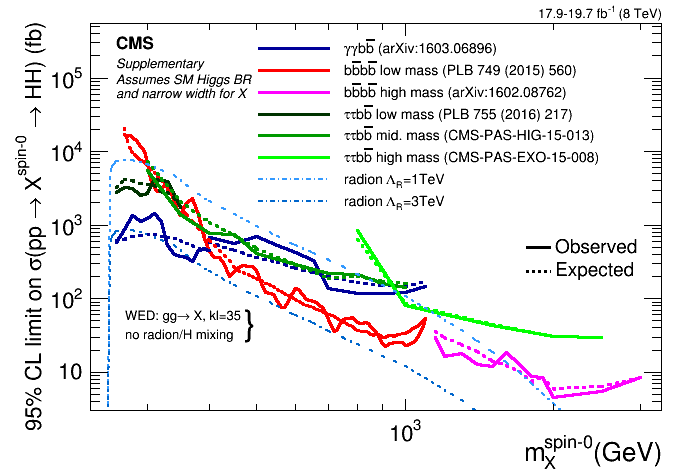
\includegraphics[width=.7\textwidth]{./Figures/CMS_spin0_exc.png}
%	\label{fig:CMS_BSMlim}
%	\caption{Exclusion limits on the mass of a spin 0 resonance from searches for Higgs pair production with the CMS detector.}
%\end{figure}

\begin{figure}
	\centering
	\begin{minipage}{.5\textwidth}
		\centering
		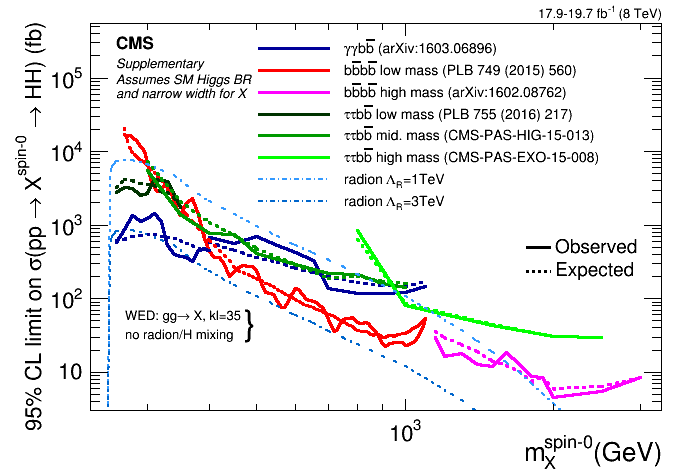
\includegraphics[width=\linewidth]{./Figures/CMS_spin0_exc.png}
	\end{minipage}%
	\begin{minipage}{.5\textwidth}
		\centering
		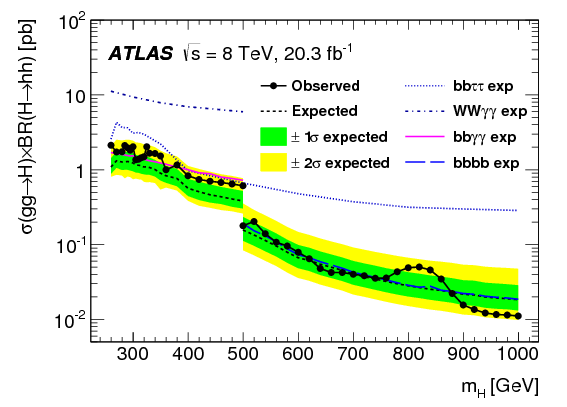
\includegraphics[width=\linewidth]{./Figures/ATLASmH.png}
	\end{minipage}
	\begin{minipage}[t]{0.5\textwidth}
		\caption*{(a)}
		%\label{fig1}
	\end{minipage}%%%
	\hfill
	\begin{minipage}[t]{0.5\textwidth}
		\caption*{(b)}
		%\label{fig2}
	\end{minipage}
	\caption{Exclusion limits (at $95\%$ CL) on the cross section of resonant Higgs pair production from the decay of heavy scalar particles. These results were obtained using proton-proton collision data collected with the CMS (a) and ATLAS (b) detector at a CM energy of $\sqrt{s}=8$ TeV and result from the combination of different channels. Plots from \cite{hhbbAA_CMS} and \cite{ATLAShhBSMcomb}.}
	\label{fig:ATLAS_CMS_BSMlim}
\end{figure}

\section{Feasibility studies for high-luminosity and future colliders}
\label{section:feasibility}

%IDEAS FOR SECTION \\
%- HL-LHC feasibility study \cite{hhFeasibility},\cite{hhFeasibility_LHC},\cite{hhFeasibility1_LHC} \\
%- FCC hh to 4b (Selvaggi et al.)  \cite{hh+jet_100TeV}, \cite{hhFeasibility1_100TeV}\\

Without any BSM contribution, the discovery of Higgs pairs production in the four b quarks final state at the LHC is highly unlikely even considering the total expected integrated luminosity of $300~\text{fb}^{-1}$. There might be evidence for this process but retrieving useful information about the value of the Higgs trilinear coupling will remain out of reach. Nonetheless, the HL-LHC as well as future colliders pose a good opportunity for the discovery and precision studies of this process. Therefore, Monte Carlo studies assessing the feasibility of searches for $hh\rightarrow b\overline{b}b\overline{b}$ at the HL-LHC and at the FCC-hh have been performed.

For the HL-LHC, a study including the $pp\rightarrow b\overline{b}b\overline{b}$, $pp\rightarrow b\overline{b}jj$, $pp\rightarrow jjjj$ and $pp\rightarrow t\overline{t}\rightarrow b\overline{b}jjjj$ backgrounds reports a significance ($S/\sqrt{B}$) of $4$ ($1.3$) for an integrated luminosity of $3000~(300)~\text{fb}^{-1}$ \cite{hhFeasibility}. The analysis is performed in three orthogonal regions (boosted, intermediate and resolved) and the reported significance is obtained from the combination of these three regions. The highest significance ($S/\sqrt{B}=2.9$) is achieved in the boosted category. In addition, the impact of pile up is evaluated. Considering a mean pile up of $80$ and making use of jet grooming techniques, a significance of $3.1$ ($1.0$) for an integrated luminosity of $3000~(300)~\text{fb}^{-1}$ is reported (also considering the three analysis regions). This work makes use of artificial neural networks (ANN's) as well as of jet substructure observables to further increase the signal-background separation. Furthermore, single Higgs backgrounds, namely $Z(\rightarrow b\overline{b})h(\rightarrow b\overline{b})$, $t\overline{t}h(\rightarrow b\overline{b})$ and $b\overline{b}h(\rightarrow b\overline{b})$, are shown to be negligible for the analysis, when compared to the dominant QCD multijet background.

ATLAS and CMS also carried out preliminary studies for the sensitivity on the trilinear coupling at the HL-LHC. Several channels have been investigated: $hh\rightarrow  b\overline{b}\gamma\gamma$, $hh\rightarrow b\overline{b} \tau^+ \tau^-$, $hh\rightarrow b\overline{b} WW^*$ and $hh\rightarrow  b\overline{b}b\overline{b}$. The $b\overline{b}\gamma\gamma$ final state is the most sensitive one. In this channel, ATLAS and CMS reported significances of $1.05\sigma$ \cite{ATLAShh2bbAA_HL} and $1.6\sigma$ \cite{CMShh2bbAA_HL}, respectively, for an integrated luminosity of $3000~\text{fb}^{-1}$. Taking, as an example, the ATLAS result, the achieved significance translates to an upper limit on the total di-Higgs cross section of approximately twice the SM value. This corresponds to an exclusion limit of $-0.8<k_{\lambda}<7.7$. The analysis conducted by ATLAS in this channel is done at generator level. The energy and momenta of the particles are smeared to simulate the detector's response. A mean pile up of $200$ is considered. No MVA techniques are employed in the analysis. 

For the $hh\rightarrow  b\overline{b}b\overline{b}$ channel, ATLAS states that a cross section $5.2$ times larger than the SM value can be excluded at $95\%$ CL, with systematic uncertainties being taken into consideration. The Higgs trilinear coupling is expected to be constrained to $-3.5<k_{\lambda}<11$. These results are based on the extrapolation of the current results obtained with the 2016 dataset, comprising an integrated luminosity of $10.1~\text{fb}^{-1}$. This study is based only on the resolved analysis documented in Ref. \cite{hh2bbbbATLAS}.

For the FCC-hh, a recent study that uses as signal sample $pp\rightarrow hhj\rightarrow b\overline{b}b\overline{b}j$ and that includes only the irreducible background $pp\rightarrow b\overline{b}b\overline{b}j$ reports a significance of $6.61$ for an integrated luminosity of $30~\text{ab}^{-1}$, considering an analysis that targets the boosted region \cite{hh+jet_100TeV}. The extra jet in the signal sample has $p_T>200$ GeV which provides the Higgs pair with a large Lorentz boost. This enhances the sensitivity to the Higgs boson self coupling because it favors highly boosted virtual Higgs bosons decaying to a pair of Higgs bosons. The analysis relies on the jet substructure observable $\tau_{21}$ and on a tight mass cut around the Higgs mass. No multivariate techniques are employed. 

A study comparing the feasibility of the search for di-Higgs production in the $b\overline{b}b\overline{b}$ in the HL-LHC and at the FCC-hh was presented in Ref. \cite{hhFeasibility1_100TeV}. Only the irreducible background is considered. For a boosted region, cut based analysis, a significance of $1.1$ is reported for an integrated luminosity of $3~\text{ab}^{-1}$ at $\sqrt{s}=14$ TeV (HL-LHC). For an integrated luminosity of $10~\text{ab}^{-1}$ at $\sqrt{s}=100$ TeV, which corresponds to the FCC-hh, this number is $5.7$. While the significance is large for the FCC-hh, the reported signal to background ratio ($S/B$) is approximately one order of magnitude smaller, which means the measurement might be more sensitive to systematic uncertainties on the backgrounds. 

\section{Hadronic calorimeter granularity studies}
\label{sec:gran}

Even before the baseline design for the FCC-hh was established, there were studies regarding the impact of the granularity of the calorimeters in the spatial resolving power of hadronic showers and on the resolution of jet mass and substructure variables. These studies targeted the development of future colliders and greatly influenced the baseline design of the FCC-hh.

The granularity of hadronic calorimeters is a key parameter for future collider detectors because it determines how well we can resolve energy deposits from pileup vertices and highly-boosted jet topologies. In Ref. \cite{FCC_HCALgran_doubleK}, the use of smaller calorimeter cells (smaller than the ones that are used in currently operating hadronic calorimeters) to resolve individual hadrons is investigated. 
\begin{figure}
	\centering
	\begin{minipage}{.5\textwidth}
		\centering
		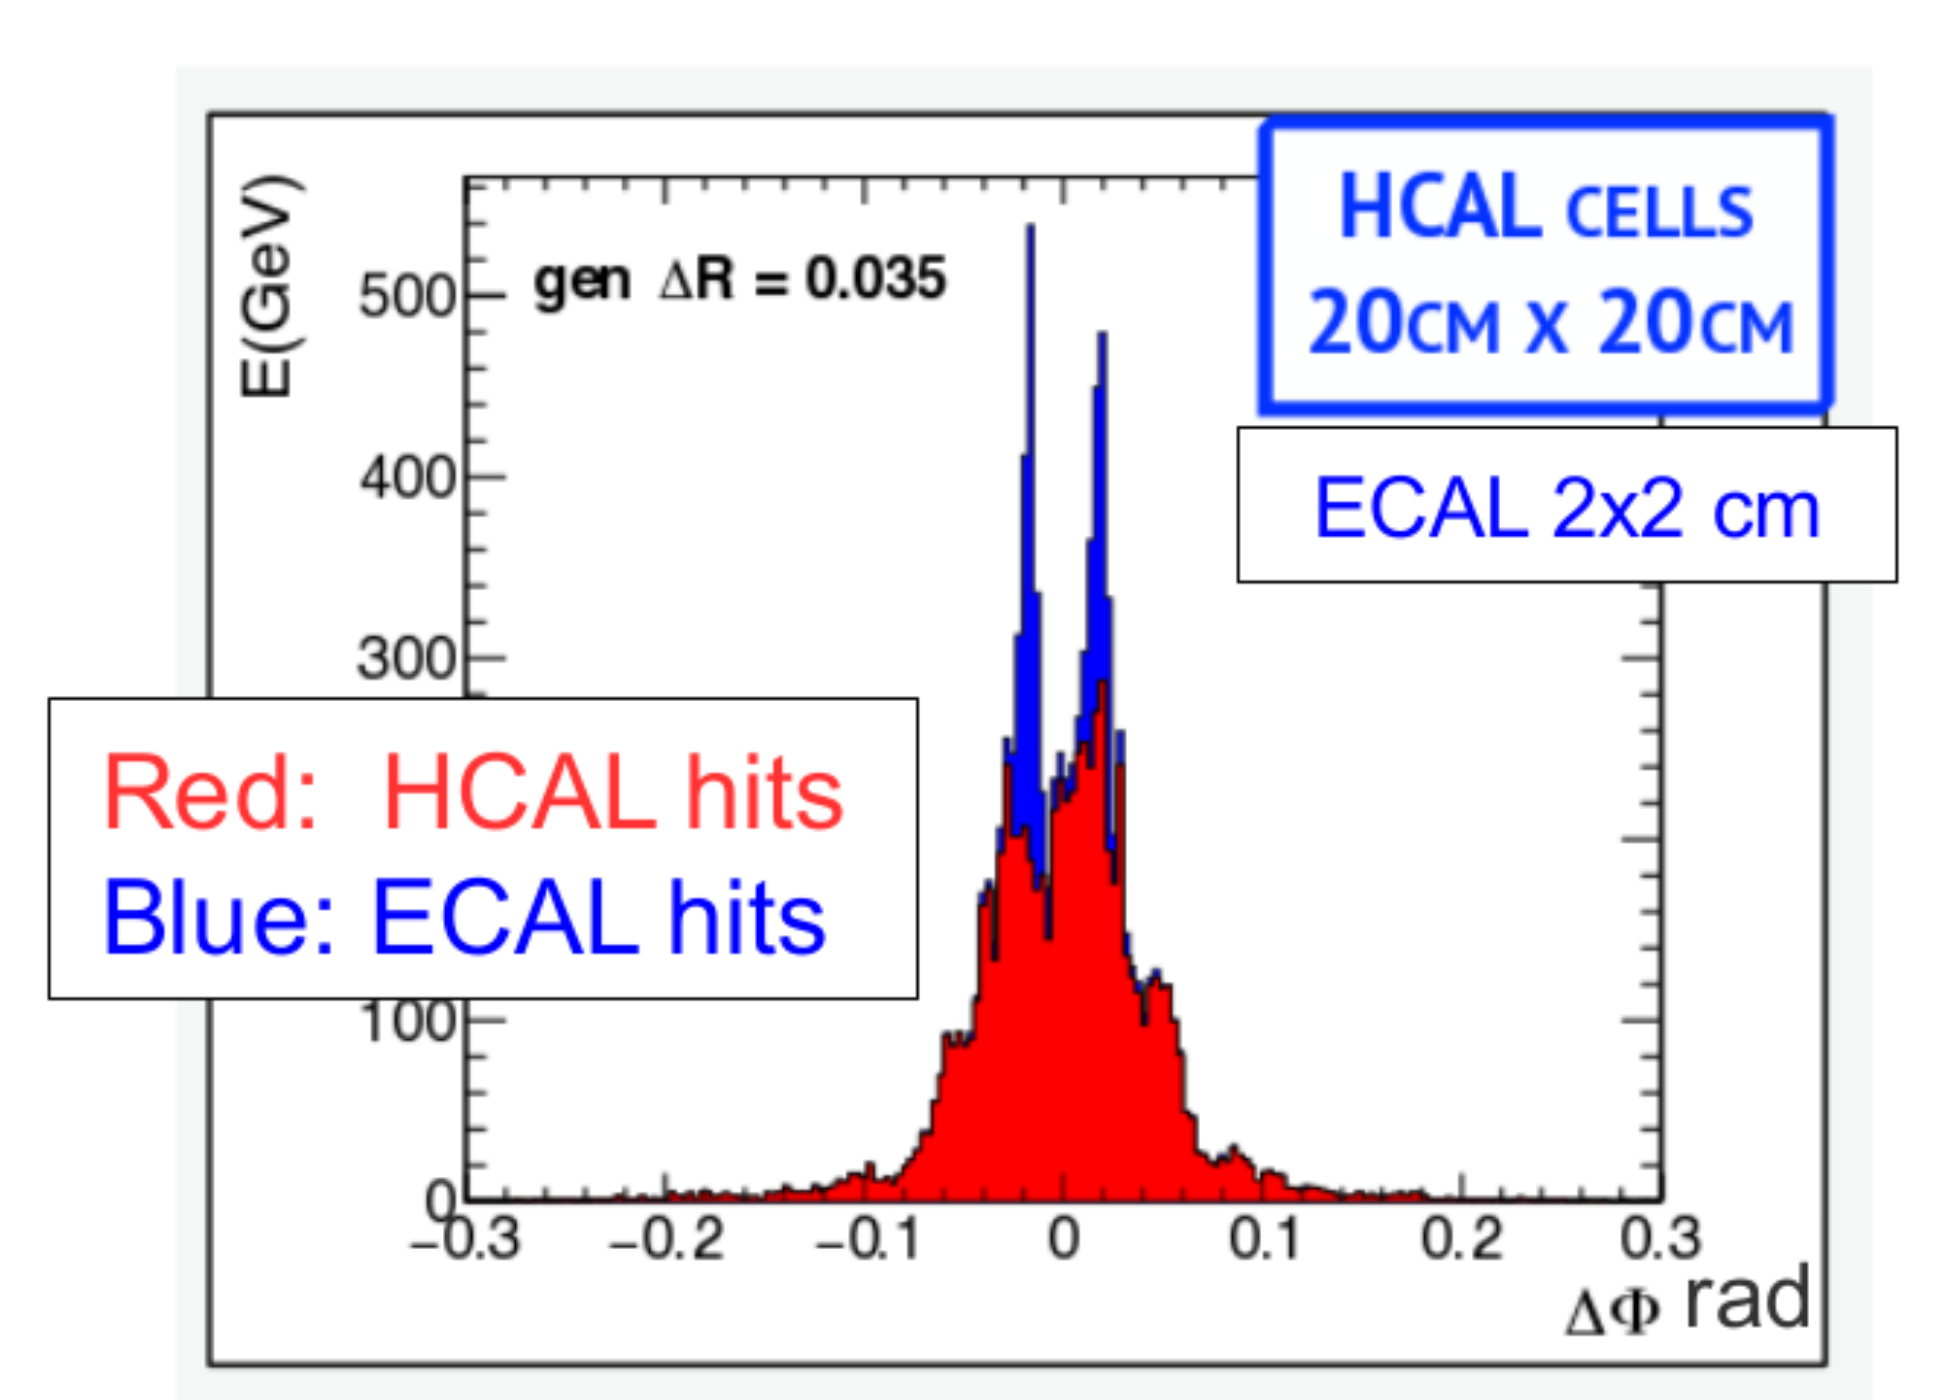
\includegraphics[trim={0 0 0 .4cm},clip,width=\linewidth]{./Figures/hcal_gran_doubleK1.png}
	\end{minipage}%
	\begin{minipage}{.5\textwidth}
		\centering
		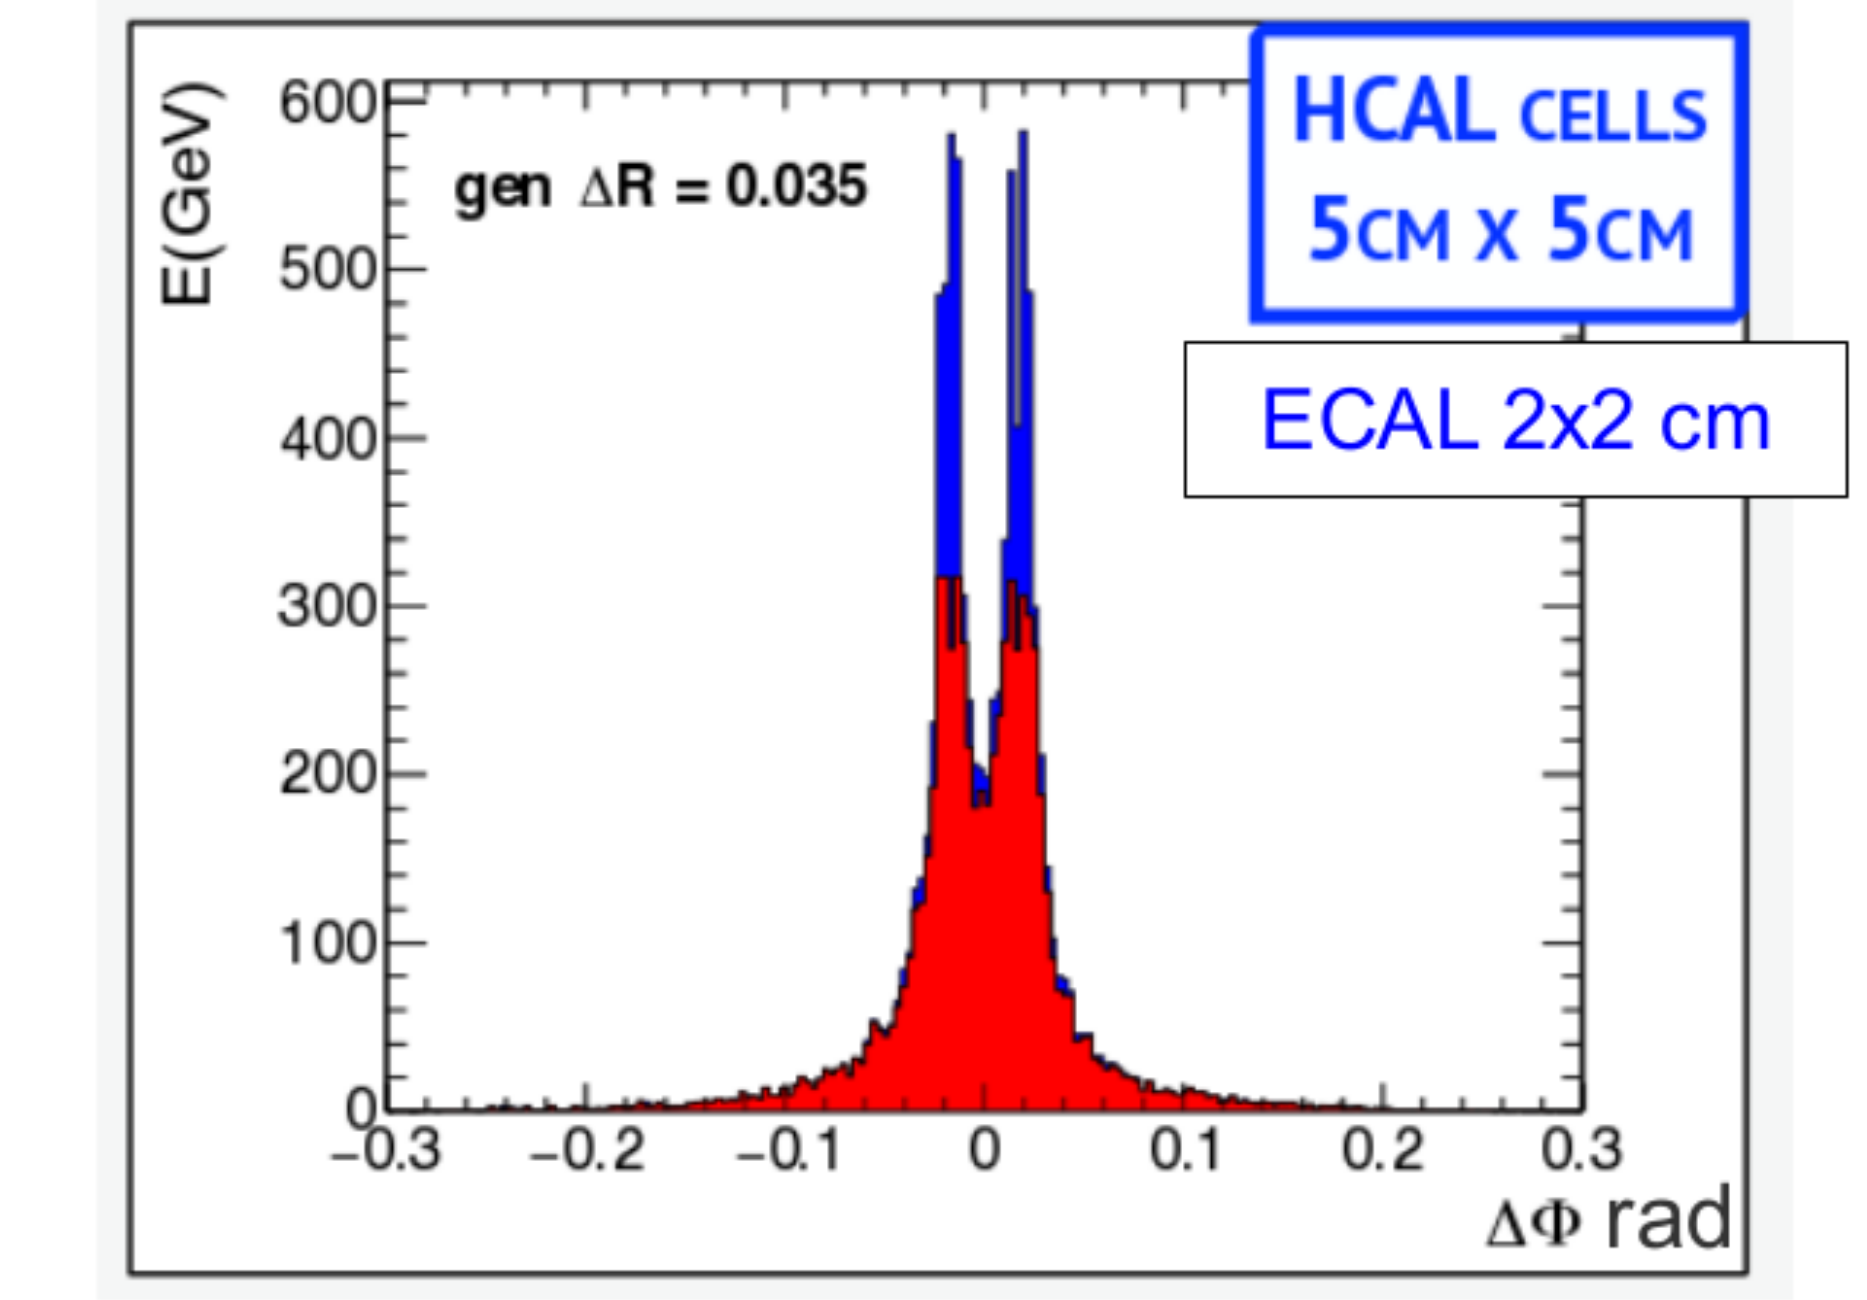
\includegraphics[width=\linewidth]{./Figures/hcal_gran_doubleK2.png}
	\end{minipage}
	\begin{minipage}[t]{0.5\textwidth}
		\caption*{(a)}
		%\label{fig1}
	\end{minipage}%%%
	\hfill
	\begin{minipage}[t]{0.5\textwidth}
		\caption*{(b)}
		%\label{fig2}
	\end{minipage}
	\caption{Azimuthal distribution of the energy deposits in the ECAL and HCAL for a pair of $K_L^0$ with $E=100$ GeV for an hadronic calorimeter with $20~\text{cm}\times 20~\text{cm}$ (a) and $5~\text{cm}\times 5~\text{cm}$ (b). Figures from \cite{BOOST2017} (based on \cite{FCC_HCALgran_doubleK}).}
	\label{fig:hcal_gran_doubleK}
\end{figure}
For two Kaons ($K_L^0$) with an energy of $100$ GeV each and with a truth level separation ($\Delta R$) equal to $0.035$ the energy deposited in the ECAL (blue) and HCAL (red) is shown as a function of $\Delta R$ for HCAL cells with sizes $20~\text{cm}\times 20~\text{cm}$ ($\Delta \eta\times \Delta\phi=0.1\times 0.1$) and $5~\text{cm}\times 5~\text{cm}$ ($\Delta \eta\times \Delta\phi=0.022\times 0.022$) in figures \ref{fig:hcal_gran_doubleK}(a) and \ref{fig:hcal_gran_doubleK}(b), respectively. The ECAL segmentation is equal to $2~\text{cm}\times 2~\text{cm}$. It is shown that for a granularity of $\Delta \eta\times \Delta\phi=0.022\times 0.022$ both hadrons can be resolved in the HCAL.

Additional studies focusing on the jet mass resolution and on the resolution of jet substructure observables were performed for three calorimeter configurations (HCAL and ECAL). Some of these studies were presented in major conferences focused on future colliders, namely FCC week 2015 and 2016 and BOOST 2017. Here, we show results presented in Refs. \cite{FCCweek2015,FCCweek2016,BOOST2017}. The calorimeter configurations tested are: HCAL(ECAL) $0.1(0.025)~\eta \times 5.6(1.4)~^{\circ}~\phi$, HCAL(ECAL) $0.05(0.012)~\eta \times 2.8(0.7)~^{\circ}~\phi$ and HCAL(ECAL) $0.025(0.006)~\eta \times 1.4(0.35)~^{\circ}~\phi$. For the segmentation in $\phi$ the numbers are give in degrees. For the HCAL, these correspond to approximately $\Delta\eta\times\Delta\phi=0.1\times0.1,0.05\times 0.05, 0.025\times0.025$. 

For $t\overline{t}$ events generated at NLO with MadGraph5 and passed through Delphes 3.2 to simulate detector response, the energy flow jet mass distribution for $p_T(\text{jet})>3$ TeV is shown in figure \ref{fig:hcal_gran_jet_mass}(a) \cite{FCCweek2015}. The jet mass resolution is shown in figure \ref{fig:hcal_gran_jet_mass}(b). For $\Delta\eta\times\Delta\phi=0.1\times0.1$ cells the root mean square (RMS) of the distribution is $0.130$. This value decreases to $0.090$ and $0.088$ for $\Delta\eta\times\Delta\phi=0.05\times0.05$ and $\Delta\eta\times\Delta\phi=0.025\times0.025$ cells, respectively. This indicates that the mass resolution increases as the granularity of the HCAL increases.

Regarding jet substructure, the resolution of the $\tau_{32}$ variable in QCD dijet events generated with Pythia8 is shown in figure \ref{fig:hcal_gran_tau32}(a) for particle flow jets \cite{FCCweek2015}. The same distribution is shown in figure \ref{fig:hcal_gran_tau32}(b) for calorimeter jets. Regardless of the type of jets used (eflow or tower jets), the $\tau_{32}$ resolution increases as the HCAL resolution increases. In addition, it is important to note that the resolution is a lot worse when using tower jets which is an indication that exploiting tracking information is vital to achieve a good resolution in substructure variables. 

Another interesting result, presented in Ref. \cite{BOOST2017}, has to do with the overlap between the $\tau_{21}$ distribution for jets resulting from QCD interactions and from the decay of a $W$ boson. Jets with $p_T$ of $2.5$ TeV show a reduction in overlap ($80\%\rightarrow 60\%$) going from $\Delta\eta\times\Delta\phi=0.1\times 0.1$ to $\Delta\eta\times\Delta\phi=0.005\times 0.005$ HCAL cells. For $5(10)$ TeV jets the overlap goes from $88(91)\%$ to $78(85)\%$. However, for $20$ TeV jets, the change in the HCAL granularity does not significantly modify the overlap, as is shown in figure \ref{fig:overlap}. 

In summary, previous studies focus on the impact of granularity in the resolution of jet mass and jet substructure observables. We did not find any studies that explored the change in the significance of a given analysis as a function of the granularity or of the detector configuration.

\begin{figure}
	\centering
	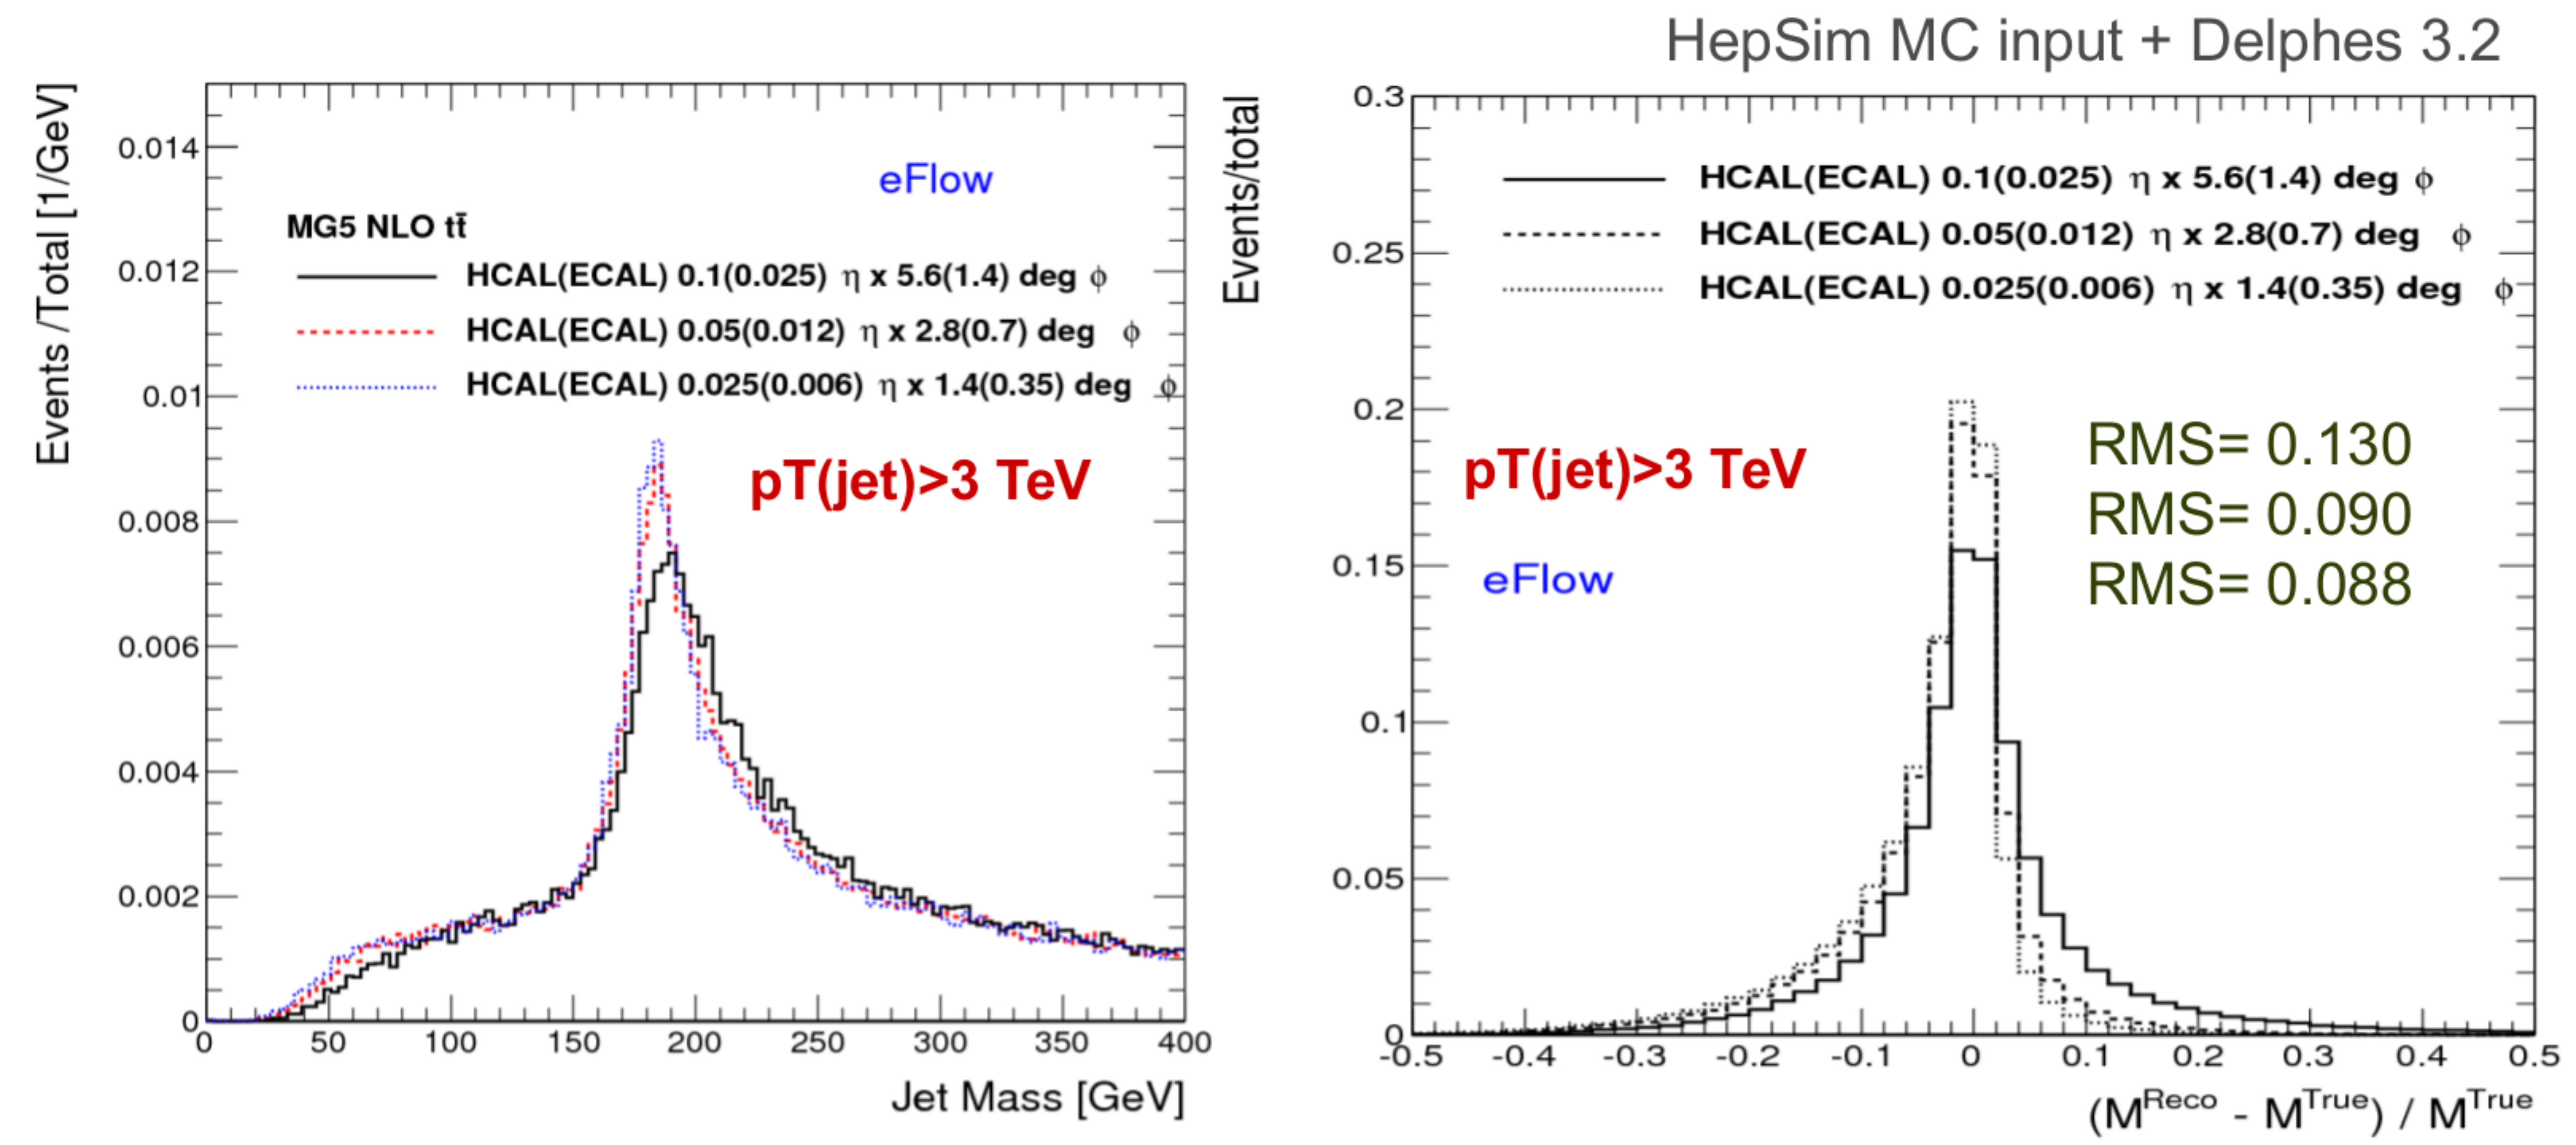
\includegraphics[width=0.9\textwidth]{./Figures/hcal_gran_jet_mass.png}
	\begin{minipage}[t]{0.45\textwidth}
		\caption*{(a)}
		%\label{fig1}
	\end{minipage}%%%
	\hfill
	\begin{minipage}[t]{0.45\textwidth}
		\caption*{(b)}
		%\label{fig2}
	\end{minipage}
	\caption{Jet mass (a) and jet mass resolution (b) plots in $t\overline{t}$ events for eflow jets with $p_T>3$ TeV for three different HCAL and ECAL configurations: HCAL(ECAL) $0.1(0.025)~\eta \times 5.6(1.4)~^{\circ}~\phi$, HCAL(ECAL) $0.05(0.012)~\eta \times 2.8(0.7)~^{\circ}~\phi$ and HCAL(ECAL) $0.025(0.006)~\eta \times 1.4(0.35)~^{\circ}~\phi$. Plots from Ref. \cite{BOOST2017}.}
	\label{fig:hcal_gran_jet_mass}
\end{figure}

\begin{figure}
	\centering
	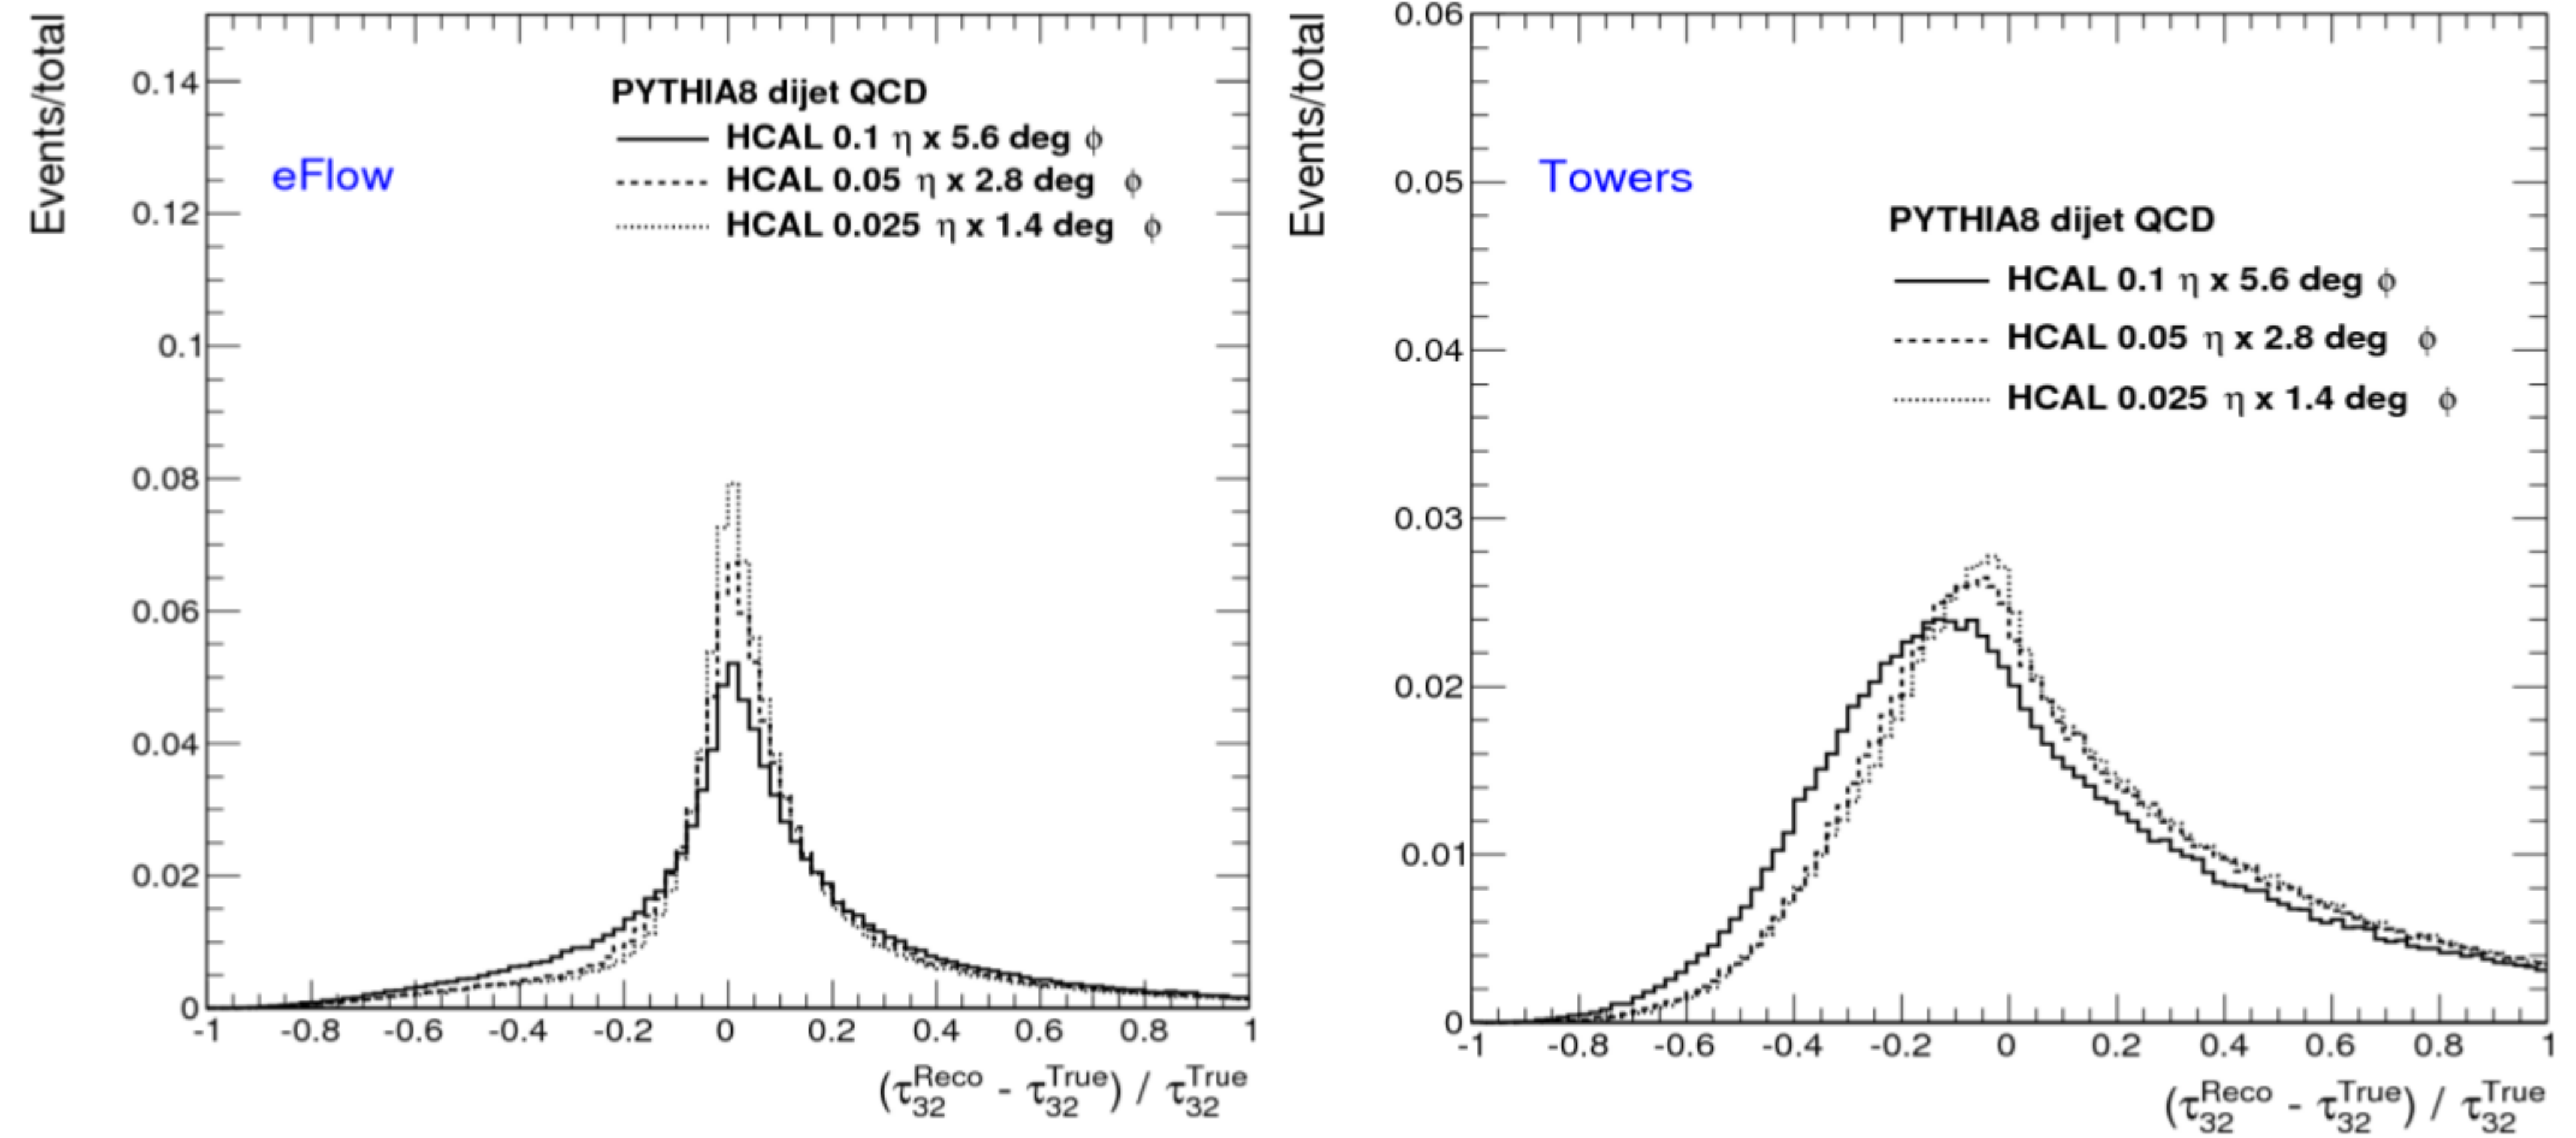
\includegraphics[width=0.9\textwidth]{./Figures/hcal_gran_tau32.png}
	\begin{minipage}[t]{0.45\textwidth}
		\caption*{(a)}
		%\label{fig1}
	\end{minipage}%%%
	\hfill
	\begin{minipage}[t]{0.45\textwidth}
		\caption*{(b)}
		%\label{fig2}
	\end{minipage}
	\caption{$\tau_{32}$ resolution plots for QCD dijet events reconstructed using eflow jets (a) and tower jets (b). Plots from Ref. \cite{FCCweek2015}.}
	\label{fig:hcal_gran_tau32}
\end{figure}

\begin{figure}
	\centering
	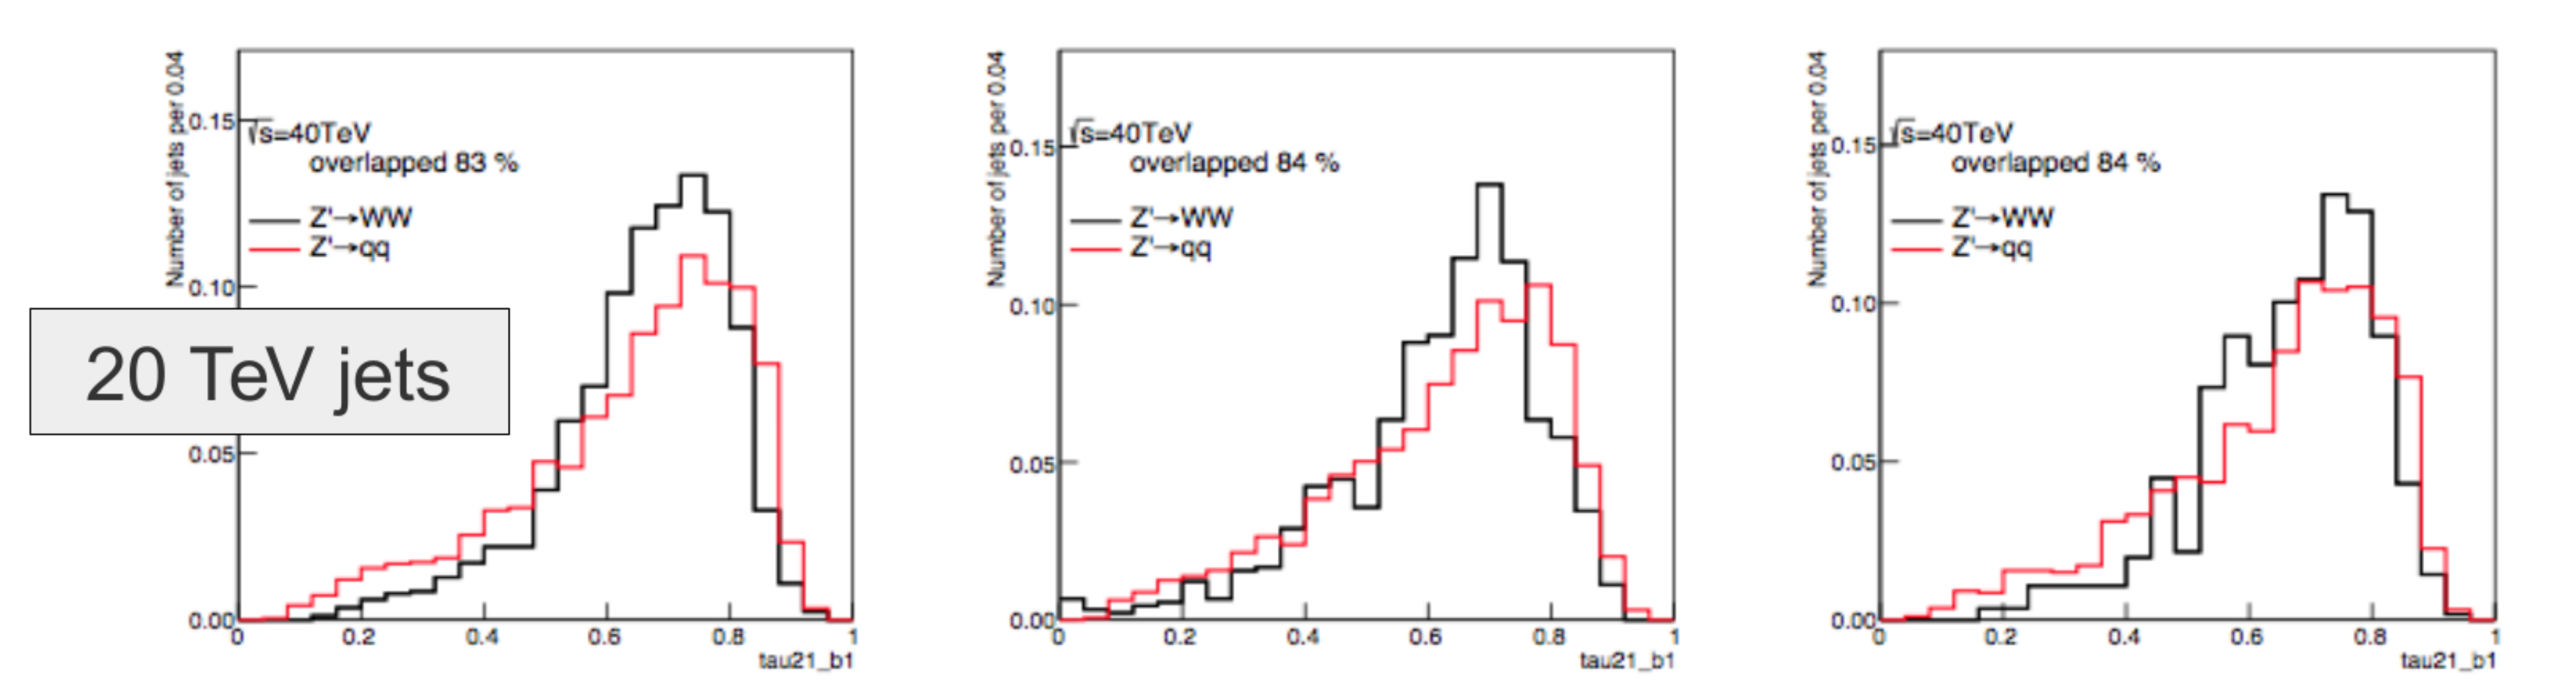
\includegraphics[width=0.9\textwidth]{./Figures/overlap.png}
	\caption{$\tau_{21}$ variable for $20$ TeV $W$ (black) and QCD jets (red) for three HCAL granularities: $\Delta\eta\times\Delta\phi=0.1\times 0.1$ (left), $\Delta\eta\times\Delta\phi=0.022\times 0.022$ (middle) and $\Delta\eta\times\Delta\phi=0.005\times 0.005$ (right). Plots from Ref. \cite{BOOST2017}.}
	\label{fig:overlap}
\end{figure}

%?? 
%IDEAS FOR SECTION\\
%- Introduce machine learning as a state of the art computational techinque very often used nowadays in physics analysis \\
%- Examples: analysis (refer back to studies presented in previous section since they both use MVAs), b tagging algorithms \\
%- Packages used: sklearn, TMVA (ROOT)\\
%- Discuss in some detail a BDT if we use it in the analysis \\
%------------------------------------------------------------------\\
%
%Machine learning techniques such as neural networks and boosted decision trees are widely used today in high energy physics. These state of the art computational techniques have proven to be useful and reliable tools to further increase the signal-background separation with respect to the traditional cut-based analysis. 
%
%Two examples of analysis employing MVA methods are the ones described in the previous section. 

